\chapter{Output}
\label{ch:output}

The standard GROMACS output (\file{.trr}, \file{.edr}, \file{.gro}, \file{.log}, \file{.cpt}) is written as usual.
The module writes into \file{simulation\_output/} in the directory \code{mdrun} runs in.
Times in the files are GROMACS times in ps unless the header says otherwise; atom indices are 0-based.

\section{Run summaries}
\label{sec:summaries}

At the first step \code{mdrun -ionize} prints a summary to stderr and the \file{.log}:
\begin{lstlisting}
 MolDStruct SF (strong-field ionization, ADK) with the trapped-electron cloud - DEVELOPMENT BUILD
 System        1960 atoms (H 959, C 613, N 193, O 185, S 10), ionization charge +0 at the start
 Pulse         0.005 J, 850 nm, FWHM 2 fs, peak at 2 fs, focus 30000 nm
               peak intensity 3.32e+17 W/cm^2, peak field 1.58e+03 V/nm
 Run           600 steps x 2 as = 1.2 fs; seed 7 (GMX_SFMD_SEED); 4 ranks

 Processes
   ADK tunnel ionization                    on (always)
   trapped electrons (Poisson-Boltzmann)    on   sfmd-electrons = pbgrid
       grid                                 s_e 0.25 nm, 2.5 cells/s_e, box <= 3 R, <= 384 cells, solve every 0.2 fs
       evaporation                          on
       laser barrier                        on: envelope field (sfmd-laser-barrier = 1)
       laser heating                        on   Drude ellipsoid, nu_ei <= 1 omega_p, surface damping A = 0
       electron-impact ionization           on   Lotz
       three-body recombination             off
       temperature floor                    1 eV: solve, evaporation, recombination at >= it
   ion-ion forces                           all pairs

 Output        simulation_output/: event logs (sfmd-detailed-output = 1), charges_over_time.bin every 50 steps;
               autostop off

 Warnings (settings outside what was tested)
   - peak intensity 3.3e+17 W/cm^2: the cloud was tested at 1e15-1e17 W/cm^2 (lysozyme, 850 nm, 15 fs)
   - sfmd-heating-surface = 0: the Mie resonance is undamped (15-19 MeV heating outliers in ~1 of 8 runs ...)
\end{lstlisting}
With a schedule the run line gives the end time and the stages are listed.
The warnings cover what the tests found to matter: the cloud without the barrier or heating, barrier mode 2, no surface
damping, a collision-rate cap other than 1, recombination mode 1, the old temperature model, a coarser solve or other
smoothing, an intensity outside $10^{15}$--$10^{17}$\,W/cm$^2$, harmonic bonds, a step above 2\,as, all pairs above 10\,000
atoms, a cut-off without long range, and a pulse that ionizes nothing.

At the end:
\begin{lstlisting}
 MolDStruct SF: end of the run at 1.2 fs (nsteps)
 Charge        total +5546, 2.830 per atom; per element: H 1.00 C 4.00 N 5.00 O 6.00 S 6.00
 Events        ADK 5525, electron impact 21, three-body recombination 0
\end{lstlisting}
followed by the cloud's lines: electrons escaped at birth, trapped, evaporated and spilled, the laser heating, the final
$N$, $Q$ and $T$, the solves, the energy ledger with \code{E\_clamped}, the impact ionizations and recombinations with the
energy they moved, and how long $T$ was below the floor.
The ADK count is the final minus the initial charge, less impact ionizations, plus recombinations: exact with any number
of ranks, with or without the event logs.
A run stopped by the autostop says so (\code{autostop 2: ion directions settled, 60.0 fs after the pulse peak}).

\section{Files}

\begin{longtable}{@{}p{0.27\textwidth}p{0.68\textwidth}@{}}
\toprule
file & content \\
\midrule
\endhead
\multicolumn{2}{@{}l}{\emph{Always (with -ionize)}}\\
\file{charges.txt} & at the end: atom (1-based) and charge; read back by \opt{sfmd-initial-charges = 1} \\
\file{masses.bin} & float32 masses, once (the element of each atom) \\
\multicolumn{2}{@{}l}{\emph{With \opt{sfmd-detailed-output = 1}}}\\
\file{pulse\_profile.txt} & every step: $t$, $I(t)$ [W/cm$^2$], $E(t)$ [V/m], pulse active (0/1) \\
\file{mean\_charge\_vs\_time.txt} & every step: $t$, mean ion charge, ionizations this step, pulse active \\
\file{charges\_over\_time.bin} & float32, one frame of all atoms every \opt{sfmd-charge-output-stride} steps; frame $k$ at
  $t_{\mathrm{init}} + k\cdot$stride$\cdot\Delta t$ with the \file{.tpr}'s $\Delta t$ and stride (a schedule rescales
  the stride to keep that spacing) \\
\file{transition\_log.txt} & per ADK event: $t$, atom, element, charge before and after, field, rate, probability,
  random number \\
\file{collisional\_log.txt} & per impact ionization or recombination (after $<$ before): $t$, atom, element, charge
  before and after, $T$, $n_e$ at the atom [cm$^{-3}$], rate, probability, random number \\
\multicolumn{2}{@{}l}{\emph{With the cloud (header lines name the columns)}}\\
\file{pb\_log.txt} & per solve: $N$, $Q$, $T$, spacing, ions outside the box, Newton and CG iterations, residual,
  wall time, mean and maximum depth, work and $\Delta U$, $K$, \code{E\_clamped}, core charge, convolutions, rebuilds,
  $T$ iterations \\
\file{laser\_log.txt} & per solve: $E_0$, $Q$, $N$, $\Delta W$, $r_s$, $R$, spilled (this solve, rounds, total),
  escaped at birth and evaporated totals, $T$, heating [eV/fs] and total, $\nu/\omega$, $|E_{\mathrm{in}}|/E_0$,
  $Z_{\mathrm{eff}}$ \\
\file{screening\_log.txt} & every 100 steps (a \emph{step} column): escaped, trapped, fraction, mean energy, $R$, Debye
  length, evaporated, $T$, pressure work \\
\file{energy\_ledger.txt} & every 100 steps: step and $t$, the cumulative ion--ion and ion--cloud jumps of charge
  changes, the field work, $K$, $N$ \\
\file{pbg\_box.txt} & the adaptive box and grid at each rebuild \\
\file{pbg\_lr.txt} & with long range: per refresh, the cut-off, smoothing, ions outside, $U_{\mathrm{lr}}$, work, and
  the error against all pairs with \env{GMX\_SFMD\_PBG\_LR\_CHECK} \\
\multicolumn{2}{@{}l}{\emph{With \opt{sfmd-autostop = 2}}}\\
\file{autostop\_dirs.txt} & per check [fs]: the median heavy-ion turn, the predicted rest, the number of ions \\
\bottomrule
\end{longtable}
The ion charges are in \file{mean\_charge\_vs\_time.txt} and \file{charges.txt}; the sample's net charge is the ion charge
minus the cloud's $N$.

\section{The summary tool}

\file{tools/sfmd\_output.py} (Python~3, numpy, matplotlib for the figures; no GROMACS) reads a run's
\file{simulation\_output/}, or the run directory holding it:
\begin{lstlisting}
sfmd_output.py summary     run/              # run, final charge states, events per element and per 5 fs, cloud, autostop
sfmd_output.py charges     run/ --every 10   # mean charge per element over time
sfmd_output.py transitions run/ --type adk,impact,recomb --atom 12 --tmin 20 --tmax 40
sfmd_output.py plot        run/ [--gif [--no-h]] [--extract]
\end{lstlisting}
\code{plot} writes \file{overview.png} (Fig.~\ref{fig:overview}); \code{--gif} an explosion movie in three views along
the sample's principal axes, coloured by charge; \code{--extract} text copies of the events and the charge frames.
In Python, \code{import sfmd\_output as so} gives \code{so.read\_events}, \code{so.read\_charges} (frame times and
charges), \code{so.elements} and \code{so.table}.

Every file goes on a time axis from what the run wrote, never as steps $\times\,\Delta t$, which is wrong under a
schedule: \file{screening\_log.txt} is timed by interpolation in \file{energy\_ledger.txt}, which has both step and time,
and the charge frames by the \file{.tpr}'s $\Delta t$ and stride read from the \file{.log}.

\begin{figure}[t]
  \centering
  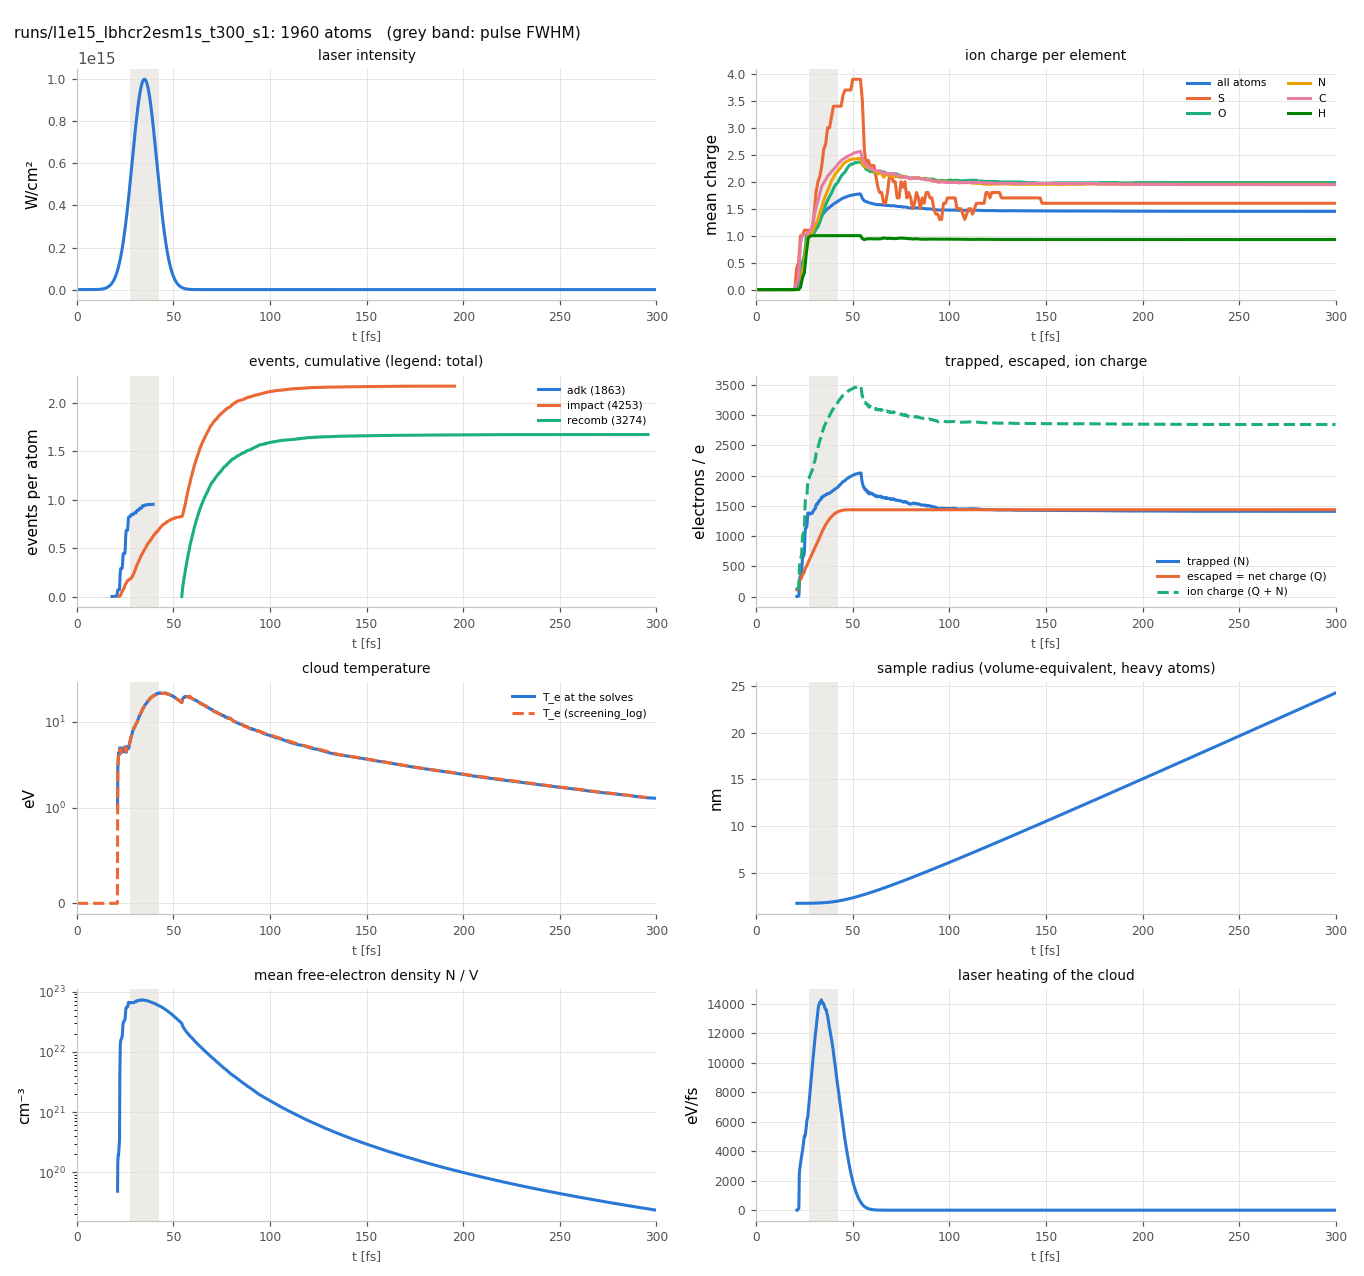
\includegraphics[width=\textwidth]{fig/overview.png}
  \caption{\code{sfmd\_output.py plot} of a lysozyme run at $10^{15}$\,W/cm$^2$ with the recommended cloud and
  recombination after the pulse, under the schedule \code{65:0.01:0.2 95:0.1:2 135:0.1:5}. The grey band is the pulse
  FWHM. The temperature from \file{screening\_log.txt} (dashed), timed through the ledger, lies on the solves' through
  the three changes of step.}
  \label{fig:overview}
\end{figure}
